\documentclass[aspectratio=169,11pt]{ctexbeamer}
\usefonttheme[onlymath]{serif}
% -----------------------------
% 基本宏包
% -----------------------------
\usepackage{amsmath,amssymb,mathtools,bm}
\usepackage{graphicx}
\usepackage{booktabs}
\usepackage{array}
\usepackage{tikz}
\usetikzlibrary{calc,decorations.pathmorphing,positioning,shapes.geometric,arrows.meta}
\usepackage{tcolorbox}
\tcbuselibrary{skins,breakable}
\usepackage{xcolor}
\usepackage{microtype}
\usepackage{hyperref}
\usepackage{pifont}     % 提供 \ding 命令（带圈数字）
\usepackage{listings}   % 代码高亮
\usepackage{tabularx}   % 选择题表格
\usepackage{ifthen}     % 条件判断
\usepackage{environ}    % \NewEnviron
\usepackage{xparse}     % 定义带多个可选参数的环境
\usepackage{etoolbox}   % \ifblank 等

% -----------------------------
% 颜色：以清爽绿色为主，轻微灰白底色
% -----------------------------
\definecolor{PrimaryGreen}{HTML}{0B7A43}
\definecolor{DeepGreen}{HTML}{085A31}
\definecolor{SoftGreen}{HTML}{EAF5EF}
\definecolor{MintGreen}{HTML}{DFF1E7}
\definecolor{WarmGray}{HTML}{666666}
\definecolor{LightGray}{HTML}{F6F7F7}
\definecolor{LineGray}{HTML}{B9BFC3}
\definecolor{TitleGray}{HTML}{2F3A3A}

% 各环境专用颜色
\definecolor{DefinitionFrame}{HTML}{0B7A43}
\definecolor{DefinitionBg}{HTML}{EAF5EF}
\definecolor{TheoremFrame}{HTML}{9B59B6}
\definecolor{TheoremBg}{HTML}{F3E5F5}
\definecolor{TipFrame}{HTML}{3498DB}
\definecolor{TipBg}{HTML}{EBF5FB}
\definecolor{ProofRed}{HTML}{C0392B}
\definecolor{ProofRedBg}{HTML}{FDEDEC}
\definecolor{RemarkFrame}{HTML}{3498DB}
\definecolor{RemarkBg}{HTML}{EBF5FB}
\definecolor{ExampleFrame}{HTML}{F1C40F}
\definecolor{ExampleBg}{HTML}{FEF9E7}
\definecolor{ExerciseFrame}{HTML}{F1C40F}
\definecolor{ExerciseBg}{HTML}{FEF9E7}

% -----------------------------
% 全局样式
% -----------------------------
\setbeamertemplate{navigation symbols}{}
\setbeamersize{text margin left=11mm, text margin right=11mm}

\setbeamerfont{structure}{series=\bfseries}
\setbeamercolor{normal text}{fg=TitleGray,bg=white}
\setbeamercolor{frametitle}{fg=PrimaryGreen,bg=white}
\setbeamercolor{title}{fg=PrimaryGreen}
\setbeamercolor{subtitle}{fg=WarmGray}
\setbeamercolor{author}{fg=TitleGray}
\setbeamercolor{date}{fg=WarmGray}

\setbeamercolor{block title}{fg=white,bg=PrimaryGreen}
\setbeamercolor{block body}{fg=TitleGray,bg=SoftGreen}
\setbeamercolor{block title alerted}{fg=white,bg=DeepGreen}
\setbeamercolor{block body alerted}{fg=TitleGray,bg=LightGray}
\setbeamercolor{itemize item}{fg=PrimaryGreen}
\setbeamercolor{itemize subitem}{fg=PrimaryGreen}
\setbeamercolor{itemize subsubitem}{fg=PrimaryGreen}
\setbeamercolor{section in toc}{fg=TitleGray}
\setbeamercolor{subsection in toc}{fg=WarmGray}

\setbeamerfont{title}{series=\bfseries,size=\LARGE}
\setbeamerfont{subtitle}{size=\large}
\setbeamerfont{frametitle}{series=\bfseries,size=\large}
\setbeamerfont{author}{size=\normalsize}
\setbeamerfont{date}{size=\normalsize}

% -----------------------------
% 项目符号风格
% -----------------------------
\setbeamertemplate{itemize item}{\small\raise0.15ex\hbox{\color{PrimaryGreen}\textbullet}}
\setbeamertemplate{itemize subitem}{\tiny\raise0.25ex\hbox{\color{PrimaryGreen}\textbullet}}
\setbeamertemplate{itemize subsubitem}{\tiny\raise0.25ex\hbox{\color{PrimaryGreen}\textbullet}}

% -----------------------------
% 页脚开关：控制短标题显示
% -----------------------------
\newif\ifshowfoottitle
\showfoottitlefalse   % 默认关闭

% -----------------------------
% 页眉/页脚
% -----------------------------
\setbeamertemplate{headline}{}
\setbeamertemplate{footline}{%
	\leavevmode
	\hbox{%
		\begin{beamercolorbox}[wd=.12\paperwidth,ht=0.72cm,dp=0.18cm,leftskip=0.25cm,rightskip=0.1cm]{}
			\color{PrimaryGreen}\rule{0.95\linewidth}{1.2pt}
		\end{beamercolorbox}
		\begin{beamercolorbox}[wd=.74\paperwidth,ht=0.72cm,dp=0.18cm,leftskip=0.15cm,rightskip=0.15cm]{}
			\ifshowfoottitle
			\usebeamerfont{title}\color{WarmGray}\insertshorttitle
			\fi
			\hfill
		\end{beamercolorbox}
		\begin{beamercolorbox}[wd=.14\paperwidth,ht=0.72cm,dp=0.18cm,center]{}
			\usebeamerfont{date}\color{WarmGray}\insertframenumber\,/\,\inserttotalframenumber
		\end{beamercolorbox}
	}
}

% -----------------------------
% frametitle 版式：左侧标题 + 右侧细线
% -----------------------------
\setbeamertemplate{frametitle}{%
	\vspace{0.15cm}
	\begin{beamercolorbox}[wd=\paperwidth,ht=1.05cm,dp=0.18cm,leftskip=0.15cm,rightskip=0.15cm]{frametitle}
		\usebeamerfont{frametitle}\color{PrimaryGreen}\insertframetitle
		\hfill
		{\color{LineGray}\rule{0.18\paperwidth}{0.6pt}}
	\end{beamercolorbox}
	\vspace{-0.1cm}
}

% -----------------------------
% 带圈数字列表（① ② ③ …）
% -----------------------------
\newcounter{quani}
\newenvironment{quan}{%
	\begin{list}{\ding{\numexpr171+\value{quani}\relax}}{%
			\usecounter{quani}%
			\setlength{\leftmargin}{2em}%
			\setlength{\labelsep}{0.5em}%
		}%
	}{%
	\end{list}%
}

\newcommand{\quannum}[1]{\ding{\numexpr171+#1\relax}\quad}

% -----------------------------
% 选择题排版
% -----------------------------
\makeatletter
\newlength{\choicelengtha}
\newlength{\choicelengthb}
\newlength{\choicelengthc}
\newlength{\choicelengthd}
\newlength{\maxlength}

\def\@optprefix{}
\def\@optsuffix{.}

\newcommand{\onech}[4]{\par
	\settowidth{\choicelengtha}{\@optprefix A\@optsuffix~#1}
	\settowidth{\choicelengthb}{\@optprefix B\@optsuffix~#2}
	\settowidth{\choicelengthc}{\@optprefix C\@optsuffix~#3}
	\settowidth{\choicelengthd}{\@optprefix D\@optsuffix~#4}
	\ifthenelse{\lengthtest{\choicelengtha>\choicelengthb}}
	{\setlength{\maxlength}{\choicelengtha}}
	{\setlength{\maxlength}{\choicelengthb}}
	\ifthenelse{\lengthtest{\choicelengthc>\maxlength}}
	{\setlength{\maxlength}{\choicelengthc}}{}
	\ifthenelse{\lengthtest{\choicelengthd>\maxlength}}
	{\setlength{\maxlength}{\choicelengthd}}{}
	\ifthenelse{\lengthtest{\maxlength>0.4\linewidth}}
	{%
		\begin{tabularx}{\linewidth}{X}
			\setlength\tabcolsep{0pt}
			\@optprefix A\@optsuffix~#1\\
			\@optprefix B\@optsuffix~#2\\
			\@optprefix C\@optsuffix~#3\\
			\@optprefix D\@optsuffix~#4\\
		\end{tabularx}
	}
	{%
		\ifthenelse{\lengthtest{\maxlength>0.2\linewidth}}
		{%
			\begin{tabularx}{\linewidth}{XX}
				\setlength\tabcolsep{0pt}
				\@optprefix A\@optsuffix~#1 & \@optprefix B\@optsuffix~#2\\
				\@optprefix C\@optsuffix~#3 & \@optprefix D\@optsuffix~#4\\
			\end{tabularx}
		}
		{%
			\begin{tabularx}{\linewidth}{XXXX}
				\setlength\tabcolsep{0pt}
				\@optprefix A\@optsuffix~#1 & \@optprefix B\@optsuffix~#2 & \@optprefix C\@optsuffix~#3 & \@optprefix D\@optsuffix~#4\\
			\end{tabularx}
		}
	}
	\unskip\unskip
}

\newcommand{\choice@A}{}
\newcommand{\choice@B}{}
\newcommand{\choice@C}{}
\newcommand{\choice@D}{}
\newcounter{choicecnt}
\newcommand{\choice@reset}{\setcounter{choicecnt}{0}}
\NewEnviron{choices}{%
	\choice@reset
	\def\choice##1{%
		\stepcounter{choicecnt}%
		\ifnum\value{choicecnt}=1 \gdef\choice@A{##1}\fi
		\ifnum\value{choicecnt}=2 \gdef\choice@B{##1}\fi
		\ifnum\value{choicecnt}=3 \gdef\choice@C{##1}\fi
		\ifnum\value{choicecnt}=4 \gdef\choice@D{##1}\fi
	}%
	\BODY
	\onech{\choice@A}{\choice@B}{\choice@C}{\choice@D}%
}
\makeatother

% -----------------------------
% 各环境专用盒子定义
% -----------------------------
\newtcolorbox{definitionbox}[1][]{%
	enhanced, breakable,
	colback=DefinitionBg,
	colframe=DefinitionFrame,
	coltitle=white,
	fonttitle=\bfseries,
	boxrule=0.55pt, arc=2.2mm,
	left=2mm, right=2mm, top=1.2mm, bottom=1.2mm,
	before skip=1.5mm, after skip=1.5mm,
	attach boxed title to top left={xshift=2mm,yshift*=-\tcboxedtitleheight/2},
	boxed title style={colback=DefinitionFrame, colframe=DefinitionFrame, arc=2.2mm, boxrule=0pt, left=2mm, right=2mm, top=1mm, bottom=1mm},
	title={#1}
}

\newtcolorbox{theorembox}[1][]{%
	enhanced, breakable,
	colback=TheoremBg,
	colframe=TheoremFrame,
	coltitle=white,
	fonttitle=\bfseries,
	boxrule=0.55pt, arc=2.2mm,
	left=2mm, right=2mm, top=1.2mm, bottom=1.2mm,
	before skip=1.5mm, after skip=1.5mm,
	attach boxed title to top left={xshift=2mm,yshift*=-\tcboxedtitleheight/2},
	boxed title style={colback=TheoremFrame, colframe=TheoremFrame, arc=2.2mm, boxrule=0pt, left=2mm, right=2mm, top=1mm, bottom=1mm},
	title={#1}
}

\newtcolorbox{proofbox}[1][]{%
	enhanced,
	breakable,
	colback=ProofRedBg,
	colframe=ProofRed,
	coltitle=white,
	fonttitle=\bfseries,
	boxrule=0.7pt,
	arc=2.2mm,
	left=2mm, right=2mm, top=1.2mm, bottom=1.2mm,
	before skip=1.5mm, after skip=1.5mm,
	title={#1},
	attach boxed title to top left={xshift=2mm,yshift*=-\tcboxedtitleheight/2},
	boxed title style={colback=ProofRed, colframe=ProofRed, arc=2.2mm, boxrule=0pt, left=2mm, right=2mm, top=1mm, bottom=1mm},
}
\tcbuselibrary{skins,breakable}
\usepackage[normalem]{ulem} % 使用 ulem 处理下划线
% -----------------------------
% 修改后的便签风格 tipbox (无需改动正文)
% -----------------------------
% 确保导言区有 \usepackage{tikz}
\newtcolorbox{tipbox}[1][提示]{%
	enhanced, 
	breakable,
	colback=white,            % 背景设为白色
	colframe=white,           % 边框透明
	fonttitle=\bfseries\color{TipFrame},
	title={#1},
	attach title to upper,    
	after title={\newline},   
	before skip=3mm, 
	after skip=3mm,
	% 使用 overlay 机制在每一行背景画线
	overlay={%
		\begin{tcbclipinterior}
			\draw[TipFrame!50, dashed, thin] 
			let \p1=(interior.south west), \p2=(interior.north west), \p3=(interior.east) 
			in 
			foreach \y in {0.5, 1.5, ..., 20} { 
				(\x1, \y1 + \y*1.2em) -- (\x3, \y1 + \y*1.2em) 
			};
		\end{tcbclipinterior}
	}
}

\newtcolorbox{remarkbox}[1][]{%
	enhanced, breakable,
	colback=RemarkBg,
	colframe=RemarkFrame,
	coltitle=white,
	fonttitle=\bfseries,
	boxrule=0.55pt, arc=2.2mm,
	left=2mm, right=2mm, top=1.2mm, bottom=1.2mm,
	before skip=1.5mm, after skip=1.5mm,
	attach boxed title to top left={xshift=2mm,yshift*=-\tcboxedtitleheight/2},
	boxed title style={colback=RemarkFrame, colframe=RemarkFrame, arc=2.2mm, boxrule=0pt, left=2mm, right=2mm, top=1mm, bottom=1mm},
	title={#1}
}

\newtcolorbox{examplebox}[1][]{%
	enhanced, breakable,
	colback=ExampleBg,
	colframe=ExampleFrame,
	coltitle=TitleGray,
	fonttitle=\bfseries,
	boxrule=0.55pt, arc=2.2mm,
	left=2mm, right=2mm, top=1.2mm, bottom=1.2mm,
	before skip=1.5mm, after skip=1.5mm,
	attach boxed title to top left={xshift=2mm,yshift*=-\tcboxedtitleheight/2},
	boxed title style={colback=ExampleFrame, colframe=ExampleFrame, arc=2.2mm, boxrule=0pt, left=2mm, right=2mm, top=1mm, bottom=1mm},
	title={#1}
}

\newtcolorbox{exercisebox}[1][]{%
	enhanced, breakable,
	colback=ExerciseBg,
	colframe=ExerciseFrame,
	coltitle=TitleGray,
	fonttitle=\bfseries,
	boxrule=0.55pt, arc=2.2mm,
	left=2mm, right=2mm, top=1.2mm, bottom=1.2mm,
	before skip=1.5mm, after skip=1.5mm,
	attach boxed title to top left={xshift=2mm,yshift*=-\tcboxedtitleheight/2},
	boxed title style={colback=ExerciseFrame, colframe=ExerciseFrame, arc=2.2mm, boxrule=0pt, left=2mm, right=2mm, top=1mm, bottom=1mm},
	title={#1}
}
% -----------------------------
% 定义思考环境 (sikao)
% -----------------------------
\newtcolorbox{sikao}[1][思考]{%
	enhanced, 
	breakable,
	beamer,
	colback=red!10,            % 背景白
	colframe=white,           % 边框透明
	borderline={0.5pt}{0pt}{red!30}, % 可选：加一个极淡的边框以区分区域
	fonttitle=\bfseries\color{red!70!black},
	title={#1},
	attach title to upper,
	after title={\newline},
	before skip=3mm, 
	after skip=3mm,
	% 在右侧绘制问号
	overlay={%
		\node[anchor=north east, red!30, font=\fontsize{40}{40}\bfseries] 
		at ([xshift=-2mm, yshift=-2mm]frame.north east) {?};
	}
}
% -----------------------------
% 基础环境定义（安全创建或重定义）
% -----------------------------
\makeatletter
\@ifundefined{definition}{%
	\newenvironment{definition}[1][定义]{\begin{definitionbox}[#1]}{\end{definitionbox}}
}{%
	\renewenvironment{definition}[1][定义]{\begin{definitionbox}[#1]}{\end{definitionbox}}
}
\@ifundefined{theorem}{%
	\newenvironment{theorem}[1][定理]{\begin{theorembox}[#1]}{\end{theorembox}}
}{%
	\renewenvironment{theorem}[1][定理]{\begin{theorembox}[#1]}{\end{theorembox}}
}
\@ifundefined{remark}{%
	\newenvironment{remark}[1][注]{\begin{remarkbox}[#1]}{\end{remarkbox}}
}{%
	\renewenvironment{remark}[1][注]{\begin{remarkbox}[#1]}{\end{remarkbox}}
}

\@ifundefined{tip}{%
	\newenvironment{tip}[1][提示]{\begin{tipbox}[#1]}{\end{tipbox}}
}{%
	\renewenvironment{tip}[1][提示]{\begin{tipbox}[#1]}{\end{tipbox}}
}
% 先确保 proof 环境不存在（避免冲突）
\let\proof\relax
\let\endproof\relax

% 全新定义 proof 环境（简洁样式，与 answer/solutions 一致）
\NewDocumentEnvironment{proof}{O{证明}}{%
	\par\medskip
	\noindent{\color{ProofRed}\bfseries #1：}%
	\par\vspace{0.3em}%
	\ignorespaces
}{%
	\par\medskip
}
\newenvironment{answer}{%
	\par\medskip
	\noindent{\color{ProofRed}\bfseries【答案】：}
	\par\vspace{0.3em}
}{%
	\par\medskip
}
\newenvironment{solutions}{%
	\par\medskip
	\noindent{\color{ProofRed}\bfseries【解析】：}
	\par\vspace{0.3em}
}{%
	\par\medskip
}
\makeatother

% -----------------------------
% 例题/练习标题（修正版：不可展开命令构建标题）
% -----------------------------
\makeatletter
\newcounter{examplectr}
\newcounter{exercisectr}
\renewcommand{\theexamplectr}{\arabic{examplectr}}
\renewcommand{\theexercisectr}{\arabic{exercisectr}}

\newcommand{\build@example@title}[6]{%
	% #1: 自动编号文本（如“例题1”）
	% #2: 年份, #3: 地区, #4: 年级, #5: 类别, #6: 题号
	\def\@titletext{#1}%
	\def\@suffix{}%
	% 年份地区部分
	\ifblank{#2}{}{\def\@partA{#2}}%
	\ifblank{#3}{}{\ifblank{#2}{\def\@partA{#3}}{\def\@partA{#2#3}}}%
	% 年级类别部分
	\ifblank{#4}{}{\def\@partB{#4}}%
	\ifblank{#5}{}{\ifblank{#4}{\def\@partB{#5}}{\def\@partB{#4#5}}}%
	% 题号部分
	\def\@partC{#6}%
	% 拼合非空块，用逗号分隔
	\ifdefvoid{\@partA}{}{\ifdefvoid{\@suffix}{}{\edef\@suffix{\@suffix, }}\edef\@suffix{\@suffix\@partA}}%
	\ifdefvoid{\@partB}{}{\ifdefvoid{\@suffix}{}{\edef\@suffix{\@suffix, }}\edef\@suffix{\@suffix\@partB}}%
	\ifblank{#6}{}{\ifdefvoid{\@suffix}{}{\edef\@suffix{\@suffix, }}\edef\@suffix{\@suffix\@partC}}%
	\ifdefvoid{\@suffix}{}{%
		\edef\@titletext{\@titletext ：(\@suffix)}%
	}%
	\gdef\@temp@title{\@titletext}%
}

\RenewDocumentEnvironment{example}{m O{} O{} O{} O{} O{}}{%
	\stepcounter{examplectr}%
	\build@example@title{例题\theexamplectr}{#2}{#3}{#4}{#5}{#6}%
	\begin{examplebox}[\@temp@title]%
	}{%
	\end{examplebox}%
}

\NewDocumentEnvironment{exercise}{m O{} O{} O{} O{} O{}}{%
	\stepcounter{exercisectr}%
	\build@example@title{练习题\theexercisectr}{#2}{#3}{#4}{#5}{#6}%
	\begin{exercisebox}[\@temp@title]%
	}{%
	\end{exercisebox}%
}
\makeatother

% -----------------------------
% 章节页：将标题放置在两条横线中间
% -----------------------------
\AtBeginSection[]{%
	\begin{frame}[plain,noframenumbering]
		\begin{tikzpicture}[remember picture,overlay]
			\fill[white] (current page.south west) rectangle (current page.north east);
			\fill[SoftGreen] (current page.south west) rectangle ($(current page.north east)+(0,-0.18\paperheight)$);
			\draw[PrimaryGreen, line width=1.1pt] 
			($(current page.center)+(-5.0cm, 1.5cm)$) -- ++(2.6cm, 0);
			\node[anchor=center, text=PrimaryGreen, font=\bfseries\Huge] 
			at (current page.center) {\insertsection};
			\draw[LineGray, line width=0.6pt] 
			($(current page.center)+(2.4cm, -1.5cm)$) -- ++(2.6cm, 0);
		\end{tikzpicture}
	\end{frame}
}

% -----------------------------
% 标题页背景：简洁建筑线稿风格
% -----------------------------
\newcommand{\TitlePageArtwork}{%
	\begin{tikzpicture}[remember picture,overlay]
		
		% =========================================================
		% 右下主视觉
		% =========================================================
		\begin{scope}[shift={($(current page.south east)+(-0.9cm,0.55cm)$)}]
			
			% -----------------------------------------------------
			% 极淡网格背景（无绿色大矩形）
			% -----------------------------------------------------
			\foreach \x in {-6.8,-6.4,...,0} {
				\draw[LineGray!12,line width=0.2pt] (\x,0) -- (\x,5.0);
			}
			
			\foreach \y in {0.4,0.8,...,4.8} {
				\draw[LineGray!12,line width=0.2pt] (-7.0,\y) -- (0,\y);
			}
			
			% =====================================================
			% 左侧：几何圆构成
			% =====================================================
			
			\draw[LineGray!45,line width=0.45pt]
			(-5.1,2.5) circle (1.55);
			
			\draw[PrimaryGreen!70,line width=0.7pt]
			(-5.1,2.5)
			++(20:0.22)
			arc[start angle=20,end angle=320,radius=0.22]
			arc[start angle=320,end angle=620,radius=0.45]
			arc[start angle=620,end angle=940,radius=0.68]
			arc[start angle=940,end angle=1280,radius=0.92];
			
			\draw[LineGray!32,line width=0.3pt]
			(-5.1,2.5)--(-3.95,3.55);
			
			\draw[LineGray!32,line width=0.3pt]
			(-5.1,2.5)--(-6.15,3.15);
			
			\draw[LineGray!32,line width=0.3pt]
			(-5.1,2.5)--(-4.0,1.45);
			
			% =====================================================
			% 中部：函数图像
			% =====================================================
			
			\begin{scope}[shift={(-1.65,0.95)}]
				
				\draw[LineGray!60,line width=0.4pt,-{Latex[length=2mm]}]
				(-1.7,0)--(1.7,0);
				
				\draw[LineGray!60,line width=0.4pt,-{Latex[length=2mm]}]
				(0,-0.4)--(0,2.2);
				
				\draw[LineGray!75,line width=0.7pt,samples=100,domain=-1.4:1.4]
				plot (\x,{0.42*sin(140*\x r)+1.1});
				
				\draw[PrimaryGreen!75,line width=0.75pt,samples=100,domain=-1.15:1.15]
				plot (\x,{0.52*(\x*\x)+0.15});
				
				\fill[PrimaryGreen!90] (0,0.15) circle (0.045);
				
			\end{scope}
			
			% =====================================================
			% 左下：几何三角结构
			% =====================================================
			
			\draw[LineGray!38,line width=0.35pt]
			(-6.5,0.65)--(-5.4,1.65)--(-4.8,0.55)--cycle;
			
			\draw[PrimaryGreen!60,line width=0.5pt]
			(-6.5,0.65)--(-4.8,0.55);
			
			\draw[LineGray!35,line width=0.3pt]
			(-5.4,1.65)--(-5.4,0.55);
			
			% =====================================================
			% 顶部公式卡片
			% =====================================================
			
			\draw[LineGray!35,line width=0.3pt,rounded corners=1pt]
			(-6.5,4.15) rectangle (-4.55,4.78);
			
			\node[font=\scriptsize,text=LineGray!85] at (-5.52,4.47)
			{$e^{i\pi}+1=0$};
			
			\draw[LineGray!35,line width=0.3pt,rounded corners=1pt]
			(-4.05,3.95) rectangle (-1.45,4.72);
			
			\node[font=\scriptsize,text=LineGray!82] at (-2.75,4.34)
			{$\displaystyle \int_a^b f(x)\,\mathrm{d}x$};
			
			% =====================================================
			% 右上抽象结构
			% =====================================================
			
			\draw[LineGray!40,line width=0.35pt]
			(-0.75,2.95) circle (0.72);
			
			\node[font=\Large\bfseries,text=PrimaryGreen!75] at (-0.75,2.95)
			{$\pi$};
			
			\draw[LineGray!25,line width=0.25pt]
			(-0.75,2.95)--(-0.1,3.4);
			
			\draw[LineGray!25,line width=0.25pt]
			(-0.75,2.95)--(-0.05,2.95);
			
			\draw[LineGray!25,line width=0.25pt]
			(-0.75,2.95)--(-0.18,2.35);
			
			% =====================================================
			% 点阵
			% =====================================================
			
			\foreach \p in {
				(-6.4,2.2),
				(-6.0,2.7),
				(-5.7,1.9),
				(-4.7,3.6),
				(-3.9,2.1),
				(-2.9,1.0),
				(-2.2,1.5),
				(-1.2,1.8),
				(-0.4,1.2)
			}{
				\fill[LineGray!40] \p circle (0.02);
			}
			
		\end{scope}
		
		% =========================================================
		% 左上 LOGO
		% =========================================================
		
		\fill[PrimaryGreen]
		($(current page.north west)+(1.0cm,-0.9cm)$)
		rectangle ++(1.55cm,-1.55cm);
		
		\node[white,font=\bfseries\Large]
		at ($(current page.north west)+(1.78cm,-1.68cm)$)
		{MATH};
		
	\end{tikzpicture}%
}
% -----------------------------
% 数学样式：强制使用显示样式与上下限
% -----------------------------
\let\oldsum\sum
\renewcommand{\sum}{\displaystyle\oldsum\limits}
\let\oldprod\prod
\renewcommand{\prod}{\displaystyle\oldprod\limits}
\let\oldlim\lim
\renewcommand{\lim}{\displaystyle\oldlim\limits}
\let\oldmax\max
\renewcommand{\max}{\displaystyle\oldmax\limits}
\let\oldmin\min
\renewcommand{\min}{\displaystyle\oldmin\limits}
\let\oldfrac\frac
\renewcommand{\frac}{\dfrac}


% -----------------------------
% 文档信息
% -----------------------------
\title[函数的奇偶性]{函数的奇偶性}
\subtitle{高中数学·必修第一册}
\author[数学组]{数学教研组}
\date[2025-09-20]{2026年5月20日}
% 设置目录显示页码，并使用圆形数字作为编号
\setbeamertemplate{sections/subsections in toc}[ball]
\setbeamertemplate{section in toc}[sections numbered]
% 如果需要明确标注页码（通常 Beamer 默认在目录页显示 section 对应的页数）
\setbeamercolor{section in toc}{fg=PrimaryGreen}
\begin{document}

	% ========== 封面 ==========
	{
		\setbeamertemplate{footline}{}
		\begin{frame}[plain,noframenumbering]
			\TitlePageArtwork
			\vspace*{1.6cm}
			\hspace*{1.25cm}
			\begin{minipage}[t]{0.50\paperwidth}
				\vspace{0.5cm}
				{\color{PrimaryGreen}\bfseries\fontsize{24}{30}\selectfont 函数的奇偶性\par}
				\vspace{0.2cm}
				{\color{WarmGray}\Large 高中数学·必修第一册\par}
				\vspace{0.2cm}
				{\color{WarmGray}\normalsize 第一课时\par}
				\vspace{0.55cm}
				{\Large Biscuits\par}
				\vspace{0.2cm}
				{\large 2025年9月20日\par}
			\end{minipage}
		\end{frame}
	}
	
	% ========== 学习目标 ==========
	\begin{frame}{本节学习目标}
		\begin{quan}
			\item 理解函数奇偶性的定义，能判断简单函数的奇偶性。
			\item 掌握奇函数、偶函数的图象特征。
			\item 掌握奇函数在 $x=0$ 处的性质。
			\item 能利用奇偶性解决求解析式、求值等问题。
		\end{quan}
		\vspace{3mm}
		\begin{tip}
			重点：奇偶性的定义与判断方法。\\
			难点：利用奇偶性求解析式、解决综合问题。
		\end{tip}
	\end{frame}
	
	% ========== 目录 ==========
	\begin{frame}{目录}
		\tableofcontents
	\end{frame}
	
	\section{情境引入}
	
	\begin{frame}{函数图形的对称美}
		\begin{center}
			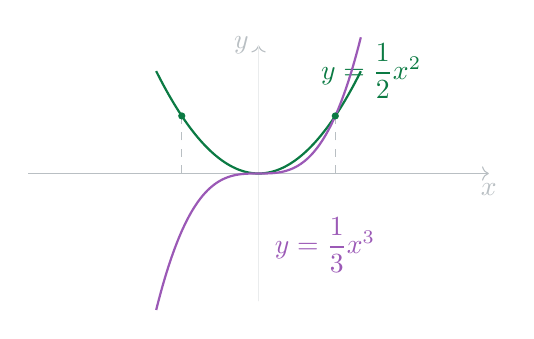
\begin{tikzpicture}[scale=0.65]
				% y轴
				\draw[->,LineGray] (-4.5,0) -- (4.5,0) node[below] {$x$};
				\draw[->,LineGray] (0,-2.5) -- (0,2.5) node[left] {$y$};
				\draw[LineGray!30] (0,-2.5) -- (0,2.5);
				% 偶函数：抛物线 y=x^2
				\draw[PrimaryGreen, thick, domain=-2:2, samples=100] plot(\x, {\x*\x/2});
				\node[PrimaryGreen] at (2.2,2) {$y=\frac12x^2$};
				% 奇函数：y=x^3/3
				\draw[TheoremFrame, thick, domain=-2:2, samples=100] plot(\x, {\x*\x*\x/3});
				\node[TheoremFrame] at (1.3,-1.4) {$y=\frac13x^3$};
				% 对称标注
				\draw[LineGray,dashed] (-1.5,0) -- (-1.5,1.125);
				\draw[LineGray,dashed] (1.5,0) -- (1.5,1.125);
				\fill[PrimaryGreen] (-1.5,1.125) circle (2pt);
				\fill[PrimaryGreen] (1.5,1.125) circle (2pt);
			\end{tikzpicture}
		\end{center}
		\begin{sikao}
			观察图象，绿色曲线关于 $y$ 轴对称，紫色曲线关于原点对称。\\
			这种对称性能否用数学式子精确描述？
		\end{sikao}
	\end{frame}
	
	\begin{frame}{从具体函数发现规律}
		\begin{columns}[T]
			\begin{column}{0.48\textwidth}
				\centering
				\textbf{探究1：$f(x)=x^2$}
				\begin{tabular}{c|c|c|c|c|c}
					\toprule
					$x$ & $-2$ & $-1$ & $0$ & $1$ & $2$ \\
					\midrule
					$f(x)$ & $4$ & $1$ & $0$ & $1$ & $4$ \\
					\bottomrule
				\end{tabular}
				\vspace{3mm}
				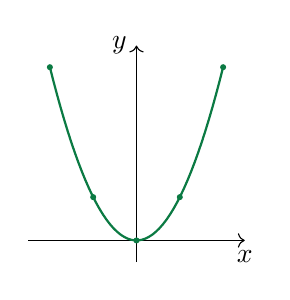
\begin{tikzpicture}[scale=0.55]
					\draw[->] (-2.5,0) -- (2.5,0) node[below] {$x$};
					\draw[->] (0,-0.5) -- (0,4.5) node[left] {$y$};
					\draw[PrimaryGreen, thick, domain=-2:2, samples=50] plot(\x, {\x*\x});
					\foreach \x in {-2,-1,0,1,2}
					\fill[PrimaryGreen] (\x, {\x*\x}) circle (2pt);
				\end{tikzpicture}
				\vspace{2mm}
				\color{PrimaryGreen} 发现：$f(-x)=f(x)$
			\end{column}
			\begin{column}{0.48\textwidth}
				\centering
				\textbf{探究2：$f(x)=x^3$}
				\begin{tabular}{c|c|c|c|c|c}
					\toprule
					$x$ & $-2$ & $-1$ & $0$ & $1$ & $2$ \\
					\midrule
					$f(x)$ & $-8$ & $-1$ & $0$ & $1$ & $8$ \\
					\bottomrule
				\end{tabular}
				\vspace{3mm}
			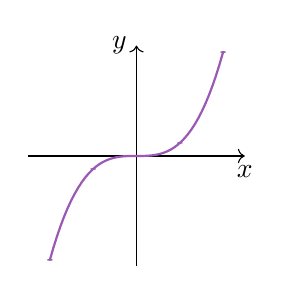
\begin{tikzpicture}[scale=0.55, yscale=0.3]  % 纵向压缩
				\draw[->] (-2.5,0) -- (2.5,0) node[below] {$x$};
				\draw[->] (0,-8.5) -- (0,8.5) node[left] {$y$};
				\draw[TheoremFrame, thick, domain=-2:2, samples=50] plot(\x, {\x*\x*\x});
				\foreach \x in {-2,-1,0,1,2}
				\fill[TheoremFrame] (\x, {\x*\x*\x}) circle (2pt);
			\end{tikzpicture}
				\vspace{2mm}
				\color{TheoremFrame} 发现：$f(-x)=-f(x)$
			\end{column}
		\end{columns}
	\end{frame}
	
	\section{定义与性质}
	
	\begin{frame}{偶函数的定义}
		\begin{definition}[偶函数]
			设函数 $f(x)$ 的定义域为 $D$，若对任意 $x\in D$，都有 $-x\in D$，且
			\[
			f(-x)=f(x),
			\]
			则称 $f(x)$ 为\textbf{偶函数}。
		\end{definition}
		\pause
		\begin{remark}
			\begin{itemize}
				\item 偶函数的图象关于 $\bm{y}$\textbf{轴}对称。
				\item 常见偶函数：$f(x)=x^2$，$f(x)=|x|$，$f(x)=\cos x$，$f(x)=c$（常数函数）。
			\end{itemize}
		\end{remark}
		\begin{tip}
			定义域关于原点对称是函数具有奇偶性的\textbf{必要条件}。
		\end{tip}
	\end{frame}
	
	\begin{frame}{奇函数的定义}
		\begin{definition}[奇函数]
			设函数 $f(x)$ 的定义域为 $D$，若对任意 $x\in D$，都有 $-x\in D$，且
			\[
			f(-x)=-f(x),
			\]
			则称 $f(x)$ 为\textbf{奇函数}。
		\end{definition}
		\pause
		\begin{remark}
			\begin{itemize}
				\item 奇函数的图象关于\textbf{原点}对称。
				\item 常见奇函数：$f(x)=x$，$f(x)=x^3$，$f(x)=\sin x$，$f(x)=\tan x$。
			\end{itemize}
		\end{remark}
	
	\end{frame}
	\begin{frame}
		\begin{sikao}
			若一个函数为奇函数，则$f(0)=$?，反之成立吗？
		\end{sikao}	
	\end{frame}
	\begin{frame}[allowframebreaks]{非奇非偶函数与既奇又偶函数}
		\begin{definition}[非奇非偶函数]
			若函数 $f(x)$ 既不满足 $f(-x)=f(x)$，也不满足 $f(-x)=-f(x)$，则称 $f(x)$ 为\textbf{非奇非偶函数}。
		\end{definition}
	
		\begin{example}{1}
			$f(x)=x^2+2x+1$ 是非奇非偶函数。\\
			验证：$f(1)=4$，$f(-1)=0$，既不等于 $f(1)$ 也不等于 $-f(1)$。
		\end{example}

		\begin{definition}[既奇又偶函数]
			若函数 $f(x)$ 同时满足 $f(-x)=f(x)$ 和 $f(-x)=-f(x)$，则称 $f(x)$ \textbf{既奇又偶}。
		\end{definition}

				\begin{theorem}
			既奇又偶的函数必为 $f(x)\equiv 0$（在定义域内恒为零），且定义域关于原点对称。
		\end{theorem}
	\end{frame}
	\section{判断方法}
	
	\begin{frame}{判断奇偶性的标准步骤}
		\begin{enumerate}
			\item \textbf{第一步：求定义域。}
			\par 判断定义域是否关于原点对称。若不对称，直接判定为\textbf{非奇非偶}。
			\item \textbf{第二步：计算 $f(-x)$。}
			\par 将解析式中所有 $x$ 替换为 $-x$，化简。
			\item \textbf{第三步：比较 $f(-x)$ 与 $f(x)$、$-f(x)$。}
			\begin{itemize}
				\item 若 $f(-x)=f(x)$ $\Rightarrow$ \textbf{偶函数}。
				\item 若 $f(-x)=-f(x)$ $\Rightarrow$ \textbf{奇函数}。
				\item 若两者均不成立 $\Rightarrow$ \textbf{非奇非偶}。
				\item 若两者均成立 $\Rightarrow$ \textbf{既奇又偶}（即 $f(x)\equiv0$）。
			\end{itemize}
		\end{enumerate}
		\begin{tip}
			判断时，先看定义域，再看解析式，缺一不可！
		\end{tip}
	\end{frame}
	
	\section{性质与证明}
	
	\begin{frame}{奇函数在原点处的性质}
		\begin{theorem}[奇函数在 $x=0$ 处的值]
			若奇函数 $f(x)$ 在 $x=0$ 处有定义，则 $f(0)=0$。
		\end{theorem}
		\pause
		\begin{proof}
			由奇函数的定义，对任意 $x$ 有 $f(-x)=-f(x)$。\\
			取 $x=0$，则 $f(0)=f(-0)=-f(0)$。\\
			移项得 $2f(0)=0$，故 $f(0)=0$。
		\end{proof}
		\pause
		\begin{remark}
			\begin{itemize}
				\item 若奇函数在 $x=0$ 处无定义（如 $f(x)=\frac1x$），则此结论不适用。
				\item 该性质常用于求参数值：若 $f(x)$ 为奇函数且定义在 $\mathbb{R}$ 上，则必有 $f(0)=0$。
			\end{itemize}
		\end{remark}
	\end{frame}
	
	\begin{frame}[allowframebreaks]{奇偶函数的运算性质}
		\begin{theorem}[四则运算的奇偶性]
			设 $f(x)$，$g(x)$ 定义域相同且关于原点对称，则：
			\begin{center}
				\begin{tabular}{c|c}
					\toprule
					运算 & 奇偶性 \\
					\midrule
					奇 $\pm$ 奇 & 奇 \\
					偶 $\pm$ 偶 & 偶 \\
					奇 $\pm$ 偶 & 非奇非偶（除非其一恒为零）\\
					奇 $\times$ 奇 & 偶 \\
					偶 $\times$ 偶 & 偶 \\
					奇 $\times$ 偶 & 奇 \\
					\bottomrule
				\end{tabular}
			\end{center}
		\end{theorem}
		\begin{proof}
			仅证"奇×奇=偶"。设 $F(x)=f(x)g(x)$，则
			\[
			F(-x)=f(-x)g(-x)=[-f(x)]\cdot[-g(x)]=f(x)g(x)=F(x).
			\]
			故 $F(x)$ 为偶函数。其余类似可证。
		\end{proof}
	\end{frame}
	
	\begin{frame}[allowframebreaks]{复合函数的奇偶性}
		\begin{theorem}[复合函数的奇偶性]
			设 $u=g(x)$，$y=f(u)$，记 $F(x)=f(g(x))$，则：
			\begin{itemize}
				\item 若 $g$ 为奇函数，$f$ 为奇函数 $\Rightarrow$ $F$ 为奇函数。
				\item 若 $g$ 为偶函数 $\Rightarrow$ $F$ 为偶函数（无论 $f$ 的奇偶性）。
				\item 若 $g$ 为奇函数，$f$ 为偶函数 $\Rightarrow$ $F$ 为偶函数。
			\end{itemize}
		\end{theorem}
		\begin{proof}
			仅证第一条。设 $g(-x)=-g(x)$，$f(-u)=-f(u)$，则
			\[
			F(-x)=f(g(-x))=f(-g(x))=-f(g(x))=-F(x).
			\]
			故 $F$ 为奇函数。
		\end{proof}
		\begin{remark}
			口诀："有偶则偶，全奇才奇"。
		\end{remark}
	\end{frame}
	
	\section{例题精讲}
	
	\begin{frame}{例题1——判断奇偶性}
		\begin{example}{1}[2025][全国卷][高一][期中][第1题]
			判断下列函数的奇偶性：
			\begin{enumerate}
				\item $f(x)=x^4-2x^2$
				\item $f(x)=x^3+x$
				\item $f(x)=\sqrt{x^2-1}$
				\item $f(x)=|x+1|-|x-1|$
			\end{enumerate}
		\end{example}
	\end{frame}
	
	\begin{frame}{例题1——解析}
	\begin{solutions}
		\begin{enumerate}
			\item 定义域 $\mathbb{R}$ 对称。$f(-x)=(-x)^4-2(-x)^2=x^4-2x^2=f(x)$，故为\textbf{偶函数}。
			\item 定义域 $\mathbb{R}$ 对称。$f(-x)=(-x)^3+(-x)=-x^3-x=-(x^3+x)=-f(x)$，故为\textbf{奇函数}。
			\item 由 $x^2-1\ge0$ 得 $x\le-1$ 或 $x\ge1$，定义域关于原点对称。
			$f(-x)=\sqrt{(-x)^2-1}=\sqrt{x^2-1}=f(x)$，故为\textbf{偶函数}。
			\item 定义域 $\mathbb{R}$ 对称。
			$f(-x)=|(-x)+1|-|(-x)-1|=|1-x|-|-x-1|$。
			又 $-f(x)=-|x+1|+|x-1|$。
			$f(1)=|2|-|0|=2$，$f(-1)=|0|-|-2|=-2$，满足 $f(-1)=-f(1)$。
			更一般地，$f(-x)=-f(x)$ 恒成立，故为\textbf{奇函数}。
		\end{enumerate}
	\end{solutions}
	\end{frame}
	
	\begin{frame}[allowframebreaks]{例题2——利用奇偶性求解析式}
		\begin{example}{4}[2025][全国][高一][月考][第2题]
			已知 $f(x)$ 是定义在 $\mathbb{R}$ 上的奇函数，且当 $x>0$ 时，$f(x)=x^2-2x$。\\
			求 $f(x)$ 在 $\mathbb{R}$ 上的解析式。
		\end{example}
		\begin{solutions}
			\begin{itemize}
				\item 当 $x>0$ 时，$f(x)=x^2-2x$（已知）。
				\item 当 $x=0$ 时，由奇函数性质 $f(0)=0$。
				\item 当 $x<0$ 时，则 $-x>0$，\\
				$f(-x)=(-x)^2-2(-x)=x^2+2x$。\\
				由奇函数定义 $f(x)=-f(-x)=-x^2-2x$。
			\end{itemize}
			综上：
			\[
			f(x)=\begin{cases}
				x^2-2x, & x>0,\\[2pt]
				0, & x=0,\\[2pt]
				-x^2-2x, & x<0.
			\end{cases}
			\]
		\end{solutions}
	\end{frame}
	
	\begin{frame}{例题3——利用奇偶性求值}
		\begin{example}{3}[2025][江苏][高一][期中][第3题]
			已知函数 $f(x)=ax^3+bx+5$，且 $f(3)=7$，求 $f(-3)$ 的值。
		\end{example}
		\pause
		\begin{solutions}
			令 $g(x)=ax^3+bx$，则 $g(x)$ 为奇函数（奇+奇=奇）。\\
			$f(x)=g(x)+5$。\\
			由 $f(3)=g(3)+5=7$，得 $g(3)=2$。\\
			由奇函数性质 $g(-3)=-g(3)=-2$。\\
			故 $f(-3)=g(-3)+5=-2+5=3$。
		\end{solutions}
		\pause
		\begin{tip}
			技巧：分离奇函数部分 $g(x)$，利用 $g(-x)=-g(x)$ 求解。
		\end{tip}
	\end{frame}
	
	\begin{frame}{例题4——奇偶性与单调性综合}
		\begin{example}{4}[2025][北京][高一][期末][第5题]
			定义在 $[-2,2]$ 上的偶函数 $f(x)$ 在 $[0,2]$ 上单调递减，且 $f(1-m)<f(m)$，求实数 $m$ 的取值范围。
		\end{example}
	\end{frame}
	
	\begin{frame}[allowframebreaks]{例题4——解析}
		\begin{solutions}
			由 $f(x)$ 为偶函数，有 $f(x)=f(|x|)$。\\
			原不等式 $f(1-m)<f(m)$ 等价于 $f(|1-m|)<f(|m|)$。\\[3mm]
			$f(x)$ 在 $[0,2]$ 上单调递减，故 $|1-m|>|m|$。\\[3mm]
			同时需满足定义域：
			\[
			\begin{cases}
				-2\le 1-m\le 2,\\
				-2\le m\le 2.
			\end{cases}
			\]
			解 $|1-m|>|m|$：平方得 $(1-m)^2>m^2\Rightarrow 1-2m>0\Rightarrow m<\dfrac12$。\\
			解定义域：$-2\le 1-m\le 2\Rightarrow -1\le m\le 3$；$-2\le m\le 2$。\\
			取交集得 $m\in[-1,2]\cap[-2,2]\cap\left(-\infty,\frac12\right)=[-1,\frac12)$。
		\end{solutions}
		\vspace{2mm}
		\color{ProofRed}\textbf{答案：$m\in[-1,\frac12)$。}
	\end{frame}
	
	\section{课堂练习}
	
	\begin{frame}{练习1——选择题}
		\begin{exercise}{1}[2025][广东][高一][期中][第1题]
			下列函数中，既是偶函数又在 $(0,+\infty)$ 上单调递增的是
		\end{exercise}
		\begin{choices}
			\choice{$y=x^3$}
			\choice{$y=|x|+1$}
			\choice{$y=-x^2$}
			\choice{$y=2^{-x}$}
		\end{choices}
	\end{frame}
	
	\begin{frame}{练习1——答案与解析}
		\begin{solutions}
			\textbf{A.} $y=x^3$ 是奇函数，$\times$\\
			\textbf{B.} $y=|x|+1$ 是偶函数，在 $(0,+\infty)$ 上 $y=x+1$ 单调递增，$\checkmark$\\
			\textbf{C.} $y=-x^2$ 是偶函数，但在 $(0,+\infty)$ 上单调递减，$\times$\\
			\textbf{D.} $y=2^{-x}$ 非奇非偶，$\times$
		\end{solutions}
		\begin{answer}
			\textbf{B}
		\end{answer}
	\end{frame}
	
	\begin{frame}{练习2——选择题}
		\begin{exercise}{2}[2025][浙江][高一][月考][第2题]
			若函数 $f(x)=\dfrac{x+a}{x^2+1}$ 为奇函数，则实数 $a$ 的值为
		\end{exercise}
		\begin{choices}
			\choice{$1$}
			\choice{$-1$}
			\choice{$0$}
			\choice{$2$}
		\end{choices}
	\end{frame}
	
	\begin{frame}{练习2——答案与解析}
		\begin{solutions}
			方法一（利用 $f(0)=0$）：\\
			$f(x)$ 定义域为 $\mathbb{R}$，由奇函数性质 $f(0)=0$，\\
			即 $\dfrac{0+a}{0^2+1}=a=0$，故 $a=0$。\\[3mm]
			方法二（利用 $f(-x)=-f(x)$）：\\
			$f(-x)=\dfrac{-x+a}{x^2+1}$，$-f(x)=-\dfrac{x+a}{x^2+1}$。\\
			由 $f(-x)=-f(x)$ 得 $-x+a=-x-a$，解得 $a=0$。
		\end{solutions}
		\begin{answer}
			\textbf{C}
		\end{answer}
	\end{frame}
	
	\begin{frame}{练习3——填空题}
		\begin{exercise}{3}[2025][山东][高一][期中][第3题]
			已知 $f(x)$ 是定义在 $\mathbb{R}$ 上的奇函数，当 $x\ge0$ 时，$f(x)=x^2+2x$，则 $f(-3)=$ \underline{\hspace{1.5cm}}。
		\end{exercise}
		\pause
		\begin{solutions}
			$f(-3)=-f(3)=-(3^2+2\times3)=-(9+6)=-15$。
		\end{solutions}
		\begin{answer}
			$-15$
		\end{answer}
	\end{frame}
	
	\begin{frame}{练习4——解答题}
		\begin{exercise}{4}[2025][全国][高一][竞赛][第4题]
			设 $f(x)$ 是定义在 $\mathbb{R}$ 上的奇函数，且对任意实数 $x$ 有 $f(x+2)=-f(x)$。
			\begin{enumerate}
				\item 证明：$f(x)$ 是以 $4$ 为周期的周期函数；
				\item 若 $f(1)=3$，求 $f(2025)$ 的值。
			\end{enumerate}
		\end{exercise}
	\end{frame}
	
	\begin{frame}{练习4——解析}
		\begin{solutions}
			\textbf{(1)} 由 $f(x+2)=-f(x)$，\\
			则 $f(x+4)=f[(x+2)+2]=-f(x+2)=-[-f(x)]=f(x)$。\\
			故 $f(x)$ 是以 $4$ 为周期的周期函数。\\[3mm]
			\textbf{(2)} $2025=4\times506+1$，\\
			由周期性 $f(2025)=f(1)=3$。
		\end{solutions}
		\begin{answer}
			(1) 见证明；(2) $f(2025)=3$
		\end{answer}
	\end{frame}
	
	\section{课堂小结}
\begin{frame}{本节知识框架}
	
	% ---------- 顶部总标题 ----------
	\begin{center}
		{\Large\bfseries\color{PrimaryGreen} 函数的奇偶性 · 知识框架}
		\vspace{2mm}
	\end{center}
	
	% ---------- 三栏布局 ----------
	\begin{columns}[T]  % [T] 表示顶部对齐
		\columnwidth\textwidth  % 强制等宽布局
		
		% ===== 第一列：定义与判断 =====
		\begin{column}{0.32\textwidth}
			\centering
			\begin{tikzpicture}[
				box/.style={draw=PrimaryGreen, fill=SoftGreen, rounded corners,
					minimum width=2.8cm, minimum height=0.75cm,
					align=center, font=\small\bfseries},
				smallbox/.style={draw=PrimaryGreen!60, fill=SoftGreen!50, rounded corners,
					minimum width=2.6cm, minimum height=0.65cm,
					align=center, font=\footnotesize},
				arrow/.style={->, >=Stealth, PrimaryGreen, thick, shorten >=1pt, shorten <=1pt}
				]
				\node[box] (t1) {定义与判断};
				\node[smallbox, below=0.5cm of t1] (i1) {偶函数：$f(-x)=f(x)$};
				\node[smallbox, below=0.3cm of i1] (i2) {奇函数：$f(-x)=-f(x)$};
				\node[smallbox, below=0.3cm of i2] (i3) {前提：定义域对称};
				\draw[arrow] (t1) -- (i1);
				\draw[arrow] (i1) -- (i2);
				\draw[arrow] (i2) -- (i3);
			\end{tikzpicture}
		\end{column}
		
		% ===== 第二列：基本性质 =====
		\begin{column}{0.32\textwidth}
			\centering
			\begin{tikzpicture}[
				box/.style={draw=PrimaryGreen, fill=SoftGreen, rounded corners,
					minimum width=2.8cm, minimum height=0.75cm,
					align=center, font=\small\bfseries},
				smallbox/.style={draw=PrimaryGreen!60, fill=SoftGreen!50, rounded corners,
					minimum width=2.6cm, minimum height=0.65cm,
					align=center, font=\footnotesize},
				arrow/.style={->, >=Stealth, PrimaryGreen, thick, shorten >=1pt, shorten <=1pt}
				]
				\node[box] (t2) {基本性质};
				\node[smallbox, below=0.5cm of t2] (j1) {四则运算的奇偶性};
				\node[smallbox, below=0.3cm of j1] (j2) {复合函数的奇偶性};
				\node[smallbox, below=0.3cm of j2] (j3) {$f(0)=0$（奇函数）};
				\draw[arrow] (t2) -- (j1);
				\draw[arrow] (j1) -- (j2);
				\draw[arrow] (j2) -- (j3);
			\end{tikzpicture}
		\end{column}
		
		% ===== 第三列：常见应用 =====
		\begin{column}{0.32\textwidth}
			\centering
			\begin{tikzpicture}[
				box/.style={draw=PrimaryGreen, fill=SoftGreen, rounded corners,
					minimum width=2.8cm, minimum height=0.75cm,
					align=center, font=\small\bfseries},
				smallbox/.style={draw=PrimaryGreen!60, fill=SoftGreen!50, rounded corners,
					minimum width=2.6cm, minimum height=0.65cm,
					align=center, font=\footnotesize},
				arrow/.style={->, >=Stealth, PrimaryGreen, thick, shorten >=1pt, shorten <=1pt}
				]
				\node[box] (t3) {常见应用};
				\node[smallbox, below=0.5cm of t3] (k1) {求函数解析式};
				\node[smallbox, below=0.3cm of k1] (k2) {求函数值};
				\node[smallbox, below=0.3cm of k2] (k3) {解不等式};
				\draw[arrow] (t3) -- (k1);
				\draw[arrow] (k1) -- (k2);
				\draw[arrow] (k2) -- (k3);
			\end{tikzpicture}
		\end{column}
	\end{columns}
	
	% ---------- 底部提示 ----------
	\vspace{5mm}
	\begin{tip}
		课后请完成配套练习册 P42--P45 相关习题。
	\end{tip}
	
\end{frame}
	\begin{frame}{课后作业}
		\begin{quan}
			\item 教材 P78 习题3.2：第1、2、3题（判断奇偶性）。
			\item 教材 P79 习题3.2：第5、6题（利用奇偶性求解析式）。
			\item 思考题：是否存在定义在 $\mathbb{R}$ 上的函数，既是奇函数又是偶函数？若有，请举例。
		\end{quan}
		\vspace{5mm}
		\begin{center}
			\color{PrimaryGreen}\rule{0.6\linewidth}{1pt}
			\vspace{2mm}
			{\large 谢谢大家！}
		\end{center}
	\end{frame}
	
	\end{document}